%\documentclass[preprint, review, 3p, authoryear]{elsarticle}
\documentclass[10pt, a4paper]{article}

%\usepackage{setspace}
\usepackage[utf8]{inputenc}
\usepackage{amsmath, amssymb, amsthm, bbm}
\usepackage{xcolor}
\usepackage{graphicx}
\usepackage[authoryear]{natbib}
\usepackage{apalike}

\DeclareMathOperator*{\argmax}{arg\,max}

\newtheorem{prob}{Problem}
\newtheorem{prop}{Proposition}
\newtheorem{definition}{Definition}

%%%%% bold symbol in math enviornment
\newcommand{\m}[1]{\boldsymbol{#1}}

\title{Merging the components of a finite mixture using  posterior probabilities}
\author{M. Comas-Cufí \and J.A. Martín-Fernández \and G. Mateu-Figueras}

%\doublespacing
\begin{document}

\maketitle

\section{Introduction}

The particular case of merging the components of a Gaussian mixture hierarchically has received special attention by different authors (see\cite{hennig2010methods} for a review of different approaches). From all different approaches presented to deal with the problem, we focus on those relying on the posterior probabilities $\tau_{ij}$, defined to be the posterior probability of observation $i$, $1 \leq i \leq n$ being generated by component $j$, $1\leq j\leq k$ after adjusting a mixture with $k$ components  to a sample $X$ with $n$ observations \citep{melnykov2013distribution,hennig2010methods,baudry2010combining,ComasCufi2013}.  Although this approaches have been presented for Gaussian mixtures, their nature allows them to be applied in any kind of probability distribution mixture.


%In general, \cite{hennig2010methods} summarises the algorithm of hierarchically merging Gaussian components as follows:
%\begin{enumerate}
%\item Start with all components of the initially estimated Gaussian mixture as current clusters
%\item Find a pair of components to merge and forming a single cluster
%%\item Calculate the posterior probability of pertinence to a cluster 
%\item Apply a stopping criterion to decide whether to merge them to form a new current cluster, or to use the current clustering as the final one.
%\item If merged, go to 2.
%\end{enumerate}

As commented, in this paper we only focus on methods based on the posterior probabilities. Our aim is to find strategies to hierachically merge components into clusters. Let us remark that we will not focus on stopping criteria, and therefore we will hierarchically merge all components until a single cluster with all components is obtained.




% \section{The subjectiveness of clustering decisions}
% 
% It is well known that there is a strong subjective component in the decision of what a ``true cluster'' is \citep{hennig2010methods}.
%
% \begin{prob}
% Given a compositional sample $T = \{ \boldsymbol{\tau_1}, \dots, \boldsymbol{\tau_n} \}$, with $\boldsymbol{\tau_i} = (\tau_{i1}, \dots, \tau_{iK})$ denoting the pertinence to classes $C_1, \dots, C_K$, build a hierarchy over the set of classes.
% \end{prob}

\section{Definitions}
\label{definitions}

Let $\mathbb{X}$ be a sample space. A \emph{finite mixture of distributions} is a probability distribution with pdf defined as the linear combination of pdf from other probability distributions all defined in $\mathbb{X}$. In general, the pdf $f$ of a finite mixture of distributions is
\begin{equation}\label{mixt}
f(\;\cdot\; ; \pi_1, \dots, \pi_k, \m\theta_1 \dots \m\theta_k) = \pi_1 f_1(\;\cdot\; ; \m\theta_1) + \dots + \pi_k f_k(\;\cdot\; ; \m\theta_k),
\end{equation}
where $\m\theta_1, \dots,  \m\theta_k$ are the parameters of the pdf $f_1, \dots, f_k$ respectively and, because $f$ is a pdf, we have the restriction $\sum_{\ell = 1}^k \pi_\ell = 1$. The probability distributions $f_j$, $1 \leq j \leq k$, are called the \emph{components} of the finite mixture $f$, or \emph{mixture components}.

Let $f$ be a finite mixture of distributions with  parameters  $\pi_1, \dots, \pi_k, \m\theta_1 \dots \m\theta_k$ as defined in Equation~\ref{mixt}, and let $I$  be a subset of $\{1, \dots, k\}$. We denote by $f_I$ the finite mixture of distributions with pdf defined by
\[
f_I = \sum_{j \in I} \frac{\pi_i}{\pi_I} f_j(\;\cdot\; ; \m\theta_j)
\]
where $\pi_I = \sum_{\ell \in I} \pi_\ell$. To simplify, we do not specify the parameters of $f_I$, which are parameters borrowed from $f$. Note that using this notation, we have that $f_{\{1, \dots, k\}} = f$ and $f_{\{j\}} = f_j$.

A \emph{partition} $\mathcal{I}$ of $\{1, \dots, k\}$ is a set of subsets of $\{1, \dots, k\}$, called $parts$, such that $\bigcup_{I \in \mathcal{I}} I = \{1, \dots, k\}$ and  if two parts $I$, $J$ are different, $I \cap J = \emptyset$ holds. To simplify, through this paper we assume an order within the elements of a partition. Doing so, we can index the partition and write $\mathcal{I} = \{ I_1, \dots, I_s\}$. Importantly, given any partition $\mathcal{I} = \{ I_1, \dots, I_s\}$, the mixture $f$ (Eq.~\ref{mixt}) can be rewritten as:
\[
f = \pi_{I_1} f_{I_1} + \dots + \pi_{I_s} f_{I_s}.
\]


A \emph{hierarchical combination of components} is a sequence of partitions $\mathcal{I}_1, \dots, \mathcal{I}_k$ of $\{1,...,k\}$, where $\mathcal{I}_1$ is the one-part partition $\mathcal{I}_1 = \{ \{1, \dots, k\} \}$, and for each $k'$, $1 <  k' \leq k$,
\begin{itemize}
\item $\mathcal{I}_{k'}$ has $k'$ elements  and
\item if a part $I \in \mathcal{I}_{k'-1}$ then either there is a part $J \in \mathcal{I}_{k'}$ with $J = I$ or there are two parts $J_1, J_2 \in \mathcal{I}_i$ with $I = J_1 \cup J_2$.
\end{itemize}


\subsection*{Model-based clustering}

When model-based clustering is based on finite mixtures, a common approach is to assume that a sample is following a finite mixture of distributions $f_1, \dots, f_k$, and then proceed as follows, 
\begin{enumerate}
\item finding a suitable estimators $\hat{\pi}_1, \dots, \hat{\pi}_k,$ $\hat{\m\theta}_1, \dots, \hat{\m\theta}_k$ of parameters $\pi_1, \dots, \pi_k,$ $\m\theta_1, \dots, \m\theta_k$, and
\item classifying each observation according to the maximum a posteriori criteria, i.e., two observations $\m x, \m y \in \mathbb{X}$ are classified to same cluster if and only if
\[
\argmax_{j=1}^k \frac{ \hat{\pi}_j f_j(\m x ; \hat{\m\theta}_j) }{\sum_{\ell=1}^k \hat{\pi}_\ell f_\ell(\m x ; \hat{\m\theta}_\ell) } = \argmax_{j=1}^k \frac{ \hat{\pi}_j f_j(\m y ; \hat{\m\theta}_j) }{ \sum_{\ell=1}^k \hat{\pi}_\ell f_\ell(\m y ; \hat{\m\theta}_\ell) }.
\]
\end{enumerate}


\cite{lee2004combining,hennig2010methods,baudry2010combining,melnykov2013distribution,pastore2013merging} noted that classifying an element according to the probability of belonging to one component could be misleading. Instead, they propose that one cluster can be formed by the combination of different mixture components. Formally, given a partition $\mathcal{I} = \{ I_1, \dots, I_s\}$, two elements $\m x, \m y \in \mathbb{X}$ are classified to the same cluster if and only if
\begin{equation}\label{cluster_criteria}
\argmax_{j=1}^s \frac{ \hat{\pi}_{I_j} \hat{f}_{I_j}(\m x) }{\sum_{\ell=1}^s \hat{\pi}_{I_\ell} \hat{f}_{I_\ell}(\m x ) } = \argmax_{j=1}^s \frac{ \hat{\pi}_{I_j} \hat{f}_{I_j}(\m y) }{ \sum_{\ell=1}^s \hat{\pi}_{I_\ell} \hat{f}_{I_\ell}(\m y) }
\end{equation}

where $\hat{f}_{I_j}(\; \cdot \;) = \sum_{j' \in I_j} \frac{\hat{\pi}_{j'}}{\hat{\pi}_{I_j}} f_{j'}(\; \cdot \; ; \hat{\m\theta}_{j'})$ and $\hat{\pi}_{I_j} =  \sum_{j' \in I_j} \hat{\pi}_{j'}$. 

Let $X = \{\m x_1\dots, \m x_n\}$ be a sample defined in $\mathbb{X}$. Along this paper, given a partition $\mathcal{I} = \{ I_1, \dots, I_s \}$ we define the posterior probability  of $\m x_i$ begin classified to $I_j$ as
\[
\hat{\tau}_{i I_j} =  \frac{ \hat{\pi}_{I_j} \hat{f}_{I_j}(\m x_i) }{\sum_{\ell=1}^s \hat{\pi}_{I_\ell} \hat{f}_{I_\ell}(\m x_i)},
\]
and, for a partition  $\mathcal{I} = \{ I_1, \dots, I_s\}$, we define the posterior probability vector
\[
\hat{\tau}_{i \mathcal{I}} = \left( \hat{\tau}_{i I_1} , \dots, \hat{\tau}_{i I_s}  \right).
\]
Note that whenever  $\mathcal{I} = \{ I_1, \dots, I_s\}$ is a partition, $\sum_{j=1}^s \hat{\tau}_{i I_j} = 1$ for $1 \leq i \leq n$.

For the sake of an example consider the following estimated Gaussian mixture

\[
\hat{f} = \sum_{j=1}^6 \hat{\pi}_j \phi(\;\cdot\; ; \hat{\m\mu}_j, \hat{\m\Sigma}_j)
\]
with parameters
{\small
\[
\begin{array}{l@{\hskip 0.1in}l@{\hskip 0.1in}c }
\hat{\pi}_1 = 0.13, & \hat{\m\mu}_1 = \left(10.8,69.17\right), & \hat{\m\Sigma}_1 = \left(
\begin{array}{cc}
36.41&1.45 \\ 
1.45&55.13 \\ 
\end{array}
\right), \\ & &\\ 
\end{array}
\]
\[
\begin{array}{l@{\hskip 0.1in}l@{\hskip 0.1in}c }
\hat{\pi}_2 = 0.09, & \hat{\m\mu}_2 = \left(32.68,22.46\right), & \hat{\m\Sigma}_2 = \left(
\begin{array}{cc}
26.76&1.07 \\ 
1.07&40.52 \\ 
\end{array}
\right), \\ & &\\ 
\end{array}
\]
\[
\begin{array}{l@{\hskip 0.1in}l@{\hskip 0.1in}c }
\hat{\pi}_3 = 0.07, & \hat{\m\mu}_3 = \left(13.65,51.91\right), & \hat{\m\Sigma}_3 = \left(
\begin{array}{cc}
33.95&1.35 \\ 
1.35&51.39 \\ 
\end{array}
\right), \\ & &\\ 
\end{array}
\]
\[
\begin{array}{l@{\hskip 0.1in}l@{\hskip 0.1in}c }
\hat{\pi}_4 = 0.16, & \hat{\m\mu}_4 = \left(83.8,4.21\right), & \hat{\m\Sigma}_4 = \left(
\begin{array}{cc}
82.27&3.28 \\ 
3.28&124.56 \\ 
\end{array}
\right), \\ & &\\ 
\end{array}
\]
\[
\begin{array}{l@{\hskip 0.1in}l@{\hskip 0.1in}c }
\hat{\pi}_5 = 0.24, & \hat{\m\mu}_5 = \left(41.28,19.51\right), & \hat{\m\Sigma}_5 = \left(
\begin{array}{cc}
55.87&2.23 \\ 
2.23&84.59 \\ 
\end{array}
\right), \\ & &\\ 
\end{array}
\]
\[
\begin{array}{l@{\hskip 0.1in}l@{\hskip 0.1in}c }
\hat{\pi}_6 = 0.32, & \hat{\m\mu}_6 = \left(24.69,66.04\right), & \hat{\m\Sigma}_6 = \left(
\begin{array}{cc}
57.85&2.3 \\ 
2.3&87.58 \\ 
\end{array}
\right), \\ & &\\ 
\end{array}
\]

}

The mixture $\hat{f}$ with $6$ components has been obtained as follows:
\begin{enumerate}
\item A sample  $X_{500}=\{\m x_1, \dots, \m x_{500}\}$ has been generated from a Gaussian mixture \emph{with 3 components}. The generation was done using the R package \textsc{MixSim}. The overlapping between components $\omega$ is a measure that defined the overlapping between components in a mixture (see Melnykov for more details). To generate sample $X_{500}$ a maximum overlapping of  $\check{\omega} = 0.01$ was fixed.
\item A Gaussian mixture \emph{with 6 components} has been fitted to sample $X_{500}$. To fit the finite mixture the R package \textsc{Rmixmod} was used.
\end{enumerate}
In Figure~\ref{ex_mixture} the sample is represented with the isodensity curves of the adjusted mixture $\hat{f}$. The estimated parameter $\hat{\mu}_j$ of each component is represented by a cross.

\begin{figure}[thbp]
\begin{center}
\begin{tabular}{cc}
 %   6 toy mixture
  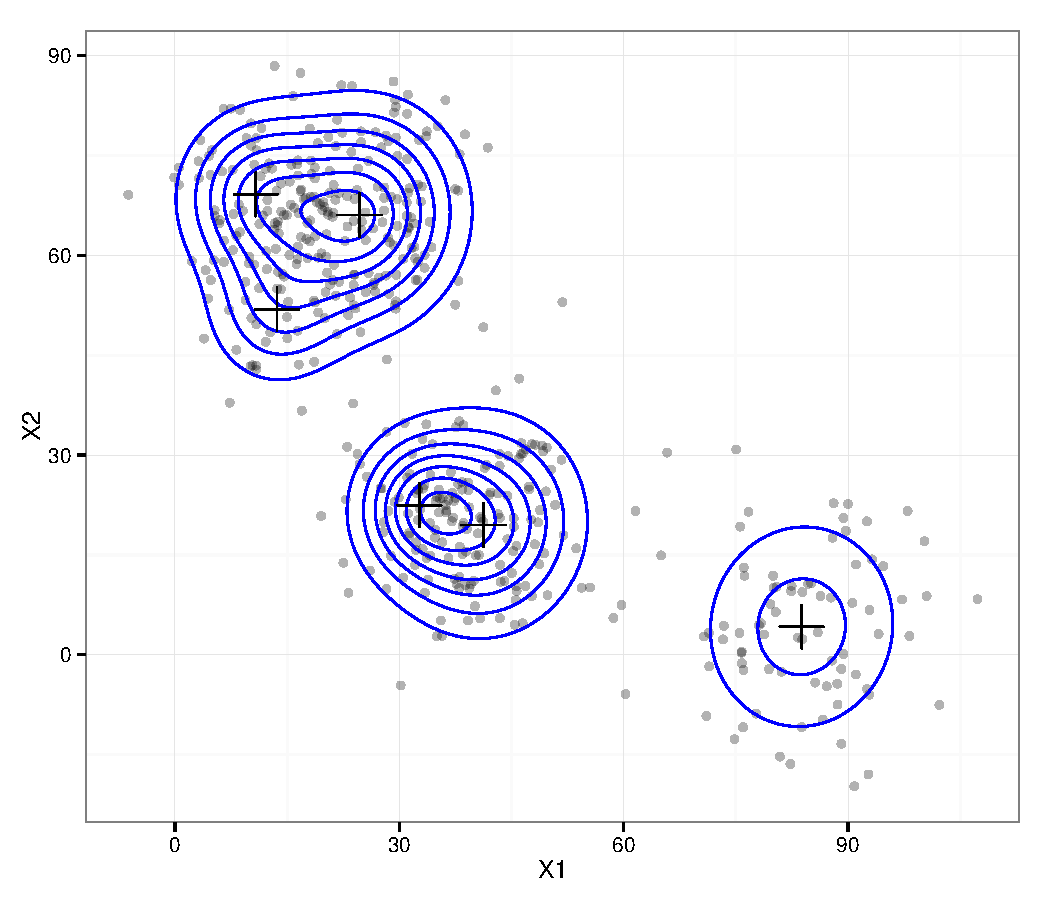
\includegraphics[trim=0cm 0cm 0cm 0cm,width=0.6\textwidth]{figures/partition-example-mixture.pdf} \\
 \end{tabular}
 \caption{Density of a Gaussian mixture with 6 component adjusted to a data set generated from a 3 component Gaussian mixture using R \textsc{MixSim} package with max overlapping of $\check{\omega} = 0.01$. Sample mean of each component is represented by '+'.}\label{ex_mixture}
\end{center}
\end{figure}

Let $I = \{1,2,3,4,5,6\}$. As commented before, any partition of $I$ yields to a feasible final classification using Eq.\ref{cluster_criteria}. For example, consider the partition 
\[\mathcal{I}_6 = \{\{1\},\{2\},\{3\},\{4\},\{5\},\{6\}\}\]
of $I$. Using partition $\mathcal{I}_6$ every observation $\m x_i \in \mathbb{R}^2$ was assigned to the part $\{j\}$ with maximum $\hat{\tau}_{i\{j\}}$. In Figure~\ref{ex_part6} each observation $\m x_i$ has been separated according to the assigned part. Moreover, the isodensity curves for each of the pdf $\hat{f}_{\{j\}} = \phi(\;\cdot\; ; \hat{\m\mu}_j, \hat{\m\Sigma}_j)$, $1\leq j \leq 6$, have been included in the graphic. 

%In other words, $\m x_i \in \mathbb{R}^2$ is assigned to cluster labeled
%\[
%\argmax_{j=1}^6 \frac{ \hat{\pi}_{\{j\}} \hat{f}_{\{j\}}(\m x) }{\sum_{\ell=1}^6 \hat{\pi}_{I_\ell} \hat{f}_{I_\ell}(\m x ) }
%\]


%$\hat{f}_{\{j\}}(\;\cdot\;) = \frac{\hat{\pi}_j}{\hat{\pi}_j} f(\;\cdot\;; \hat{\m\mu}_j, \hat{\m\Sigma}_j) = f(\;\cdot\;; \hat{\m\mu}_j, \hat{\m\Sigma}_j)$ for $j = 1,...,6$. Partition $\mathcal{I}_6$ yields to the cluster algorithm where an element $x_i$ is assigned to the part $\{j\}$ of $\mathcal{I}_6$ such that $\hat{\tau}_{i\{j\}}$ is maximum.


\begin{figure}[!h]
\begin{center}
\begin{tabular}{cc}
 %   6 toy mixture
  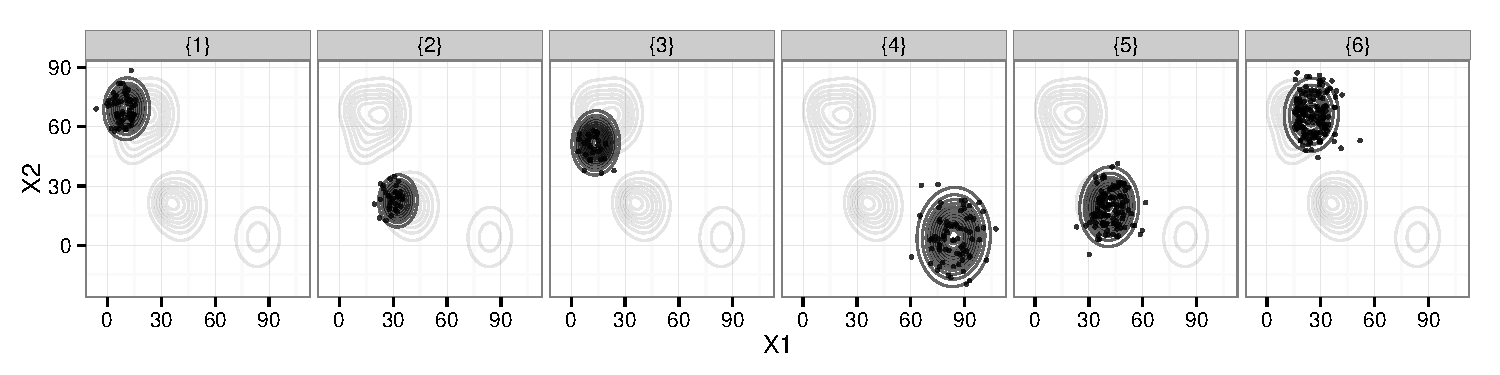
\includegraphics[trim=0cm 0cm 0cm 0cm,width=\textwidth]{figures/partition-example-part6.pdf} \\
 \end{tabular}
 \caption{ Initial classifIation with 6 clusters: each observation was assigned to a single component.}\label{ex_part6}
\end{center}
\end{figure}

In contrast, if we consider the partition
\[\mathcal{I}_3 = \{\{1, 3, 6\},\{2, 5\},\{4\}\}\]
which is grouping those components with closest mean, we get the 3 clusters given in Figure~\ref{ex_part3a}. We have included the isodensity curves of pdf $\hat{f}_{\{1,3,6\}}$, $\hat{f}_{\{2, 5\}}$ and $\hat{f}_{\{4\}}$ given by

\[ 
%\left\{ 
\begin{array}{r c l}
\hat{f}_{\{1,3,6\}} & = & \frac{1}{0.52}(0.13 \phi(\;\cdot\; ; \hat{\m\mu}_1, \hat{\m\Sigma}_1) + 0.07 \phi(\;\cdot\; ; \hat{\m\mu}_3, \hat{\m\Sigma}_3) + 0.32 \phi(\;\cdot\; ; \hat{\m\mu}_6, \hat{\m\Sigma}_6)), \\
\hat{f}_{\{2, 5\}} & = &  \frac{1}{0.33}(0.09 \phi(\;\cdot\; ; \hat{\m\mu}_2, \hat{\m\Sigma}_2) + 0.24 \phi(\;\cdot\; ; \hat{\m\mu}_5, \hat{\m\Sigma}_5)), \\
\hat{f}_{\{4\}} & = &\phi(\;\cdot\; ; \hat{\m\mu}_4, \hat{\m\Sigma}_4).
\end{array} 
%\right. 
\]
  


\begin{figure}[!h]
\begin{center}
\begin{tabular}{cc}
  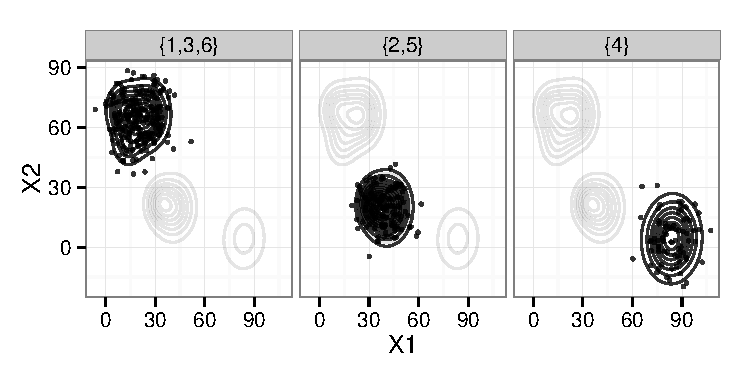
\includegraphics[trim=0cm 0cm 0cm 0cm,width=0.6\textwidth]{figures/partition-example-part3a.pdf} \\
 \end{tabular}
 \caption{Classifying assigning each observation to a single component}\label{ex_part3a}
\end{center}
\end{figure}

%Finally, suppose that instead of grouping by similar mean, we decide to group by similar covariance matrix. By choosing partition
%\[\mathcal{I}'_3 = \{\{1, 2, 3\},\{4\},\{5, 6\}\},\]
%we end up with the clustering given in Figure~\ref{ex_part3b}.
%
%\begin{figure}[!h]
%\begin{center}
%\begin{tabular}{cc}
%  \includegraphics[trim=0cm 0cm 0cm 0cm,width=0.6\textwidth]{figures/partition-example-part3b.pdf} \\
% \end{tabular}
% \caption{Classifying assigning each observation to a single component}\label{ex_part3b}
%\end{center}
%\end{figure}

Consider the following hierarchical combination of components given by the following sequence of partitions
\begin{equation}
\begin{array}{r c c}
\mathcal{H}(\mathcal{I}) &=& \{ \{\{1\},\{2\},\{3\},\{4\},\{5\},\{6\}\}, \\
   & & \{\{1, 6\},\{2\},\{3\},\{4\},\{5\} \}, \\
   & &    \{\{1, 6, 3\},\{2\},\{4\},\{5\} \}, \\
   & &    \{\{1, 6, 3\},\{2, 5\},\{4 \} \}, \\
    & &   \{\{1, 6, 3\},\{2, 4, 5\} \}, \\
   & &    \{\{1, 2, 3, 4, 5, 6\}\} \}.
\end{array}
\label{hier_ex}
\end{equation}
Each partition belonging to the hierarchical combination of components given by \ref{hier_ex} defines a clustering where each element is classified to one of the parts of each partition. Therefore, a hierarchical combination of components defines a hierarchical clustering structure. Figure~\ref{hierarchical} show that each partition defines a clustering on sample $X$. The first partition $\{\{1\},\{2\},\{3\},\{4\},\{5\},\{6\}\}$ defines a clustering with 6 clusters, the partition $\{\{1, 6\}, \{3\},\{2\},\{4\},\{5\} \}$ defines a clustering with 5 clusters, and so on.

\begin{figure}[thbp]
\begin{center}
\begin{tabular}{cc}
  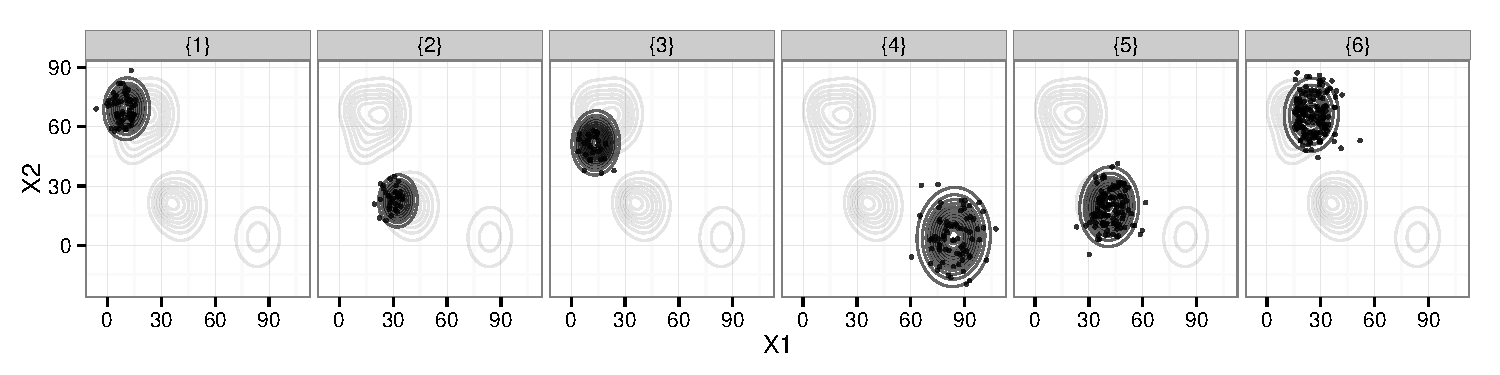
\includegraphics[trim=0cm 0cm 0cm 0cm,width=\textwidth]{figures/partition-example-part6.pdf} \\
    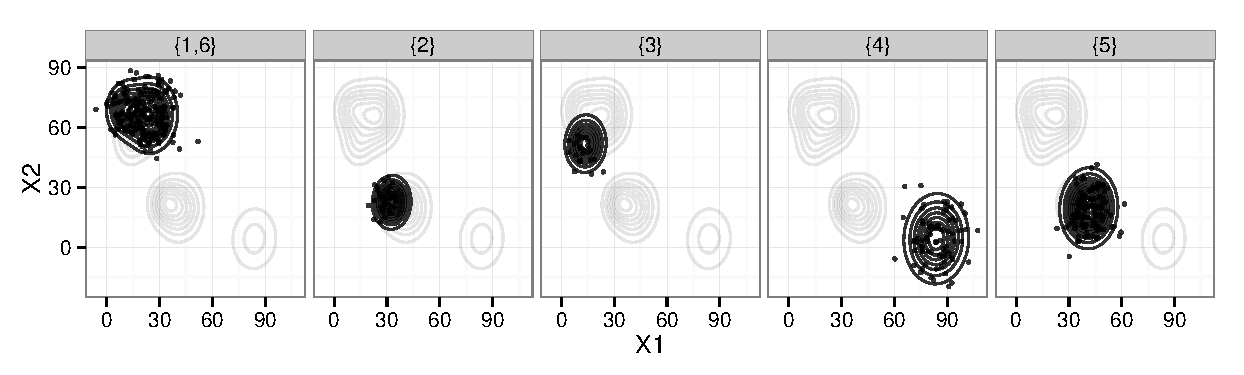
\includegraphics[trim=0cm 0cm 0cm 0cm,width=0.83\textwidth]{figures/partition-example-part5.pdf} \\
      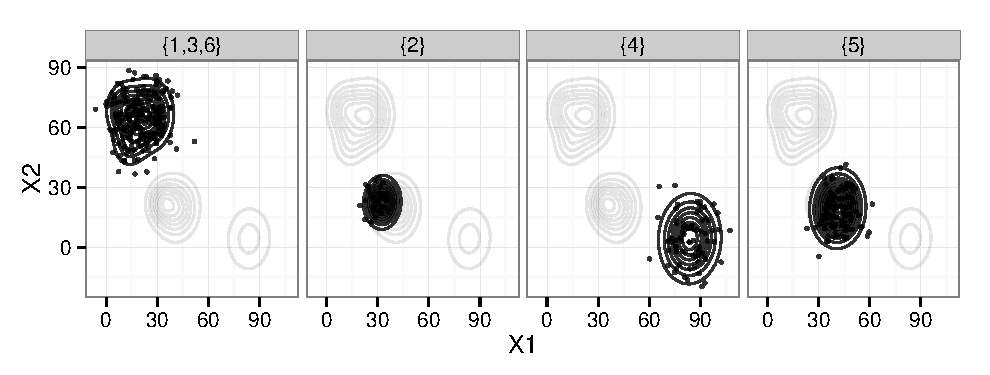
\includegraphics[trim=0cm 0cm 0cm 0cm,width=0.67\textwidth]{figures/partition-example-part4.pdf} \\
        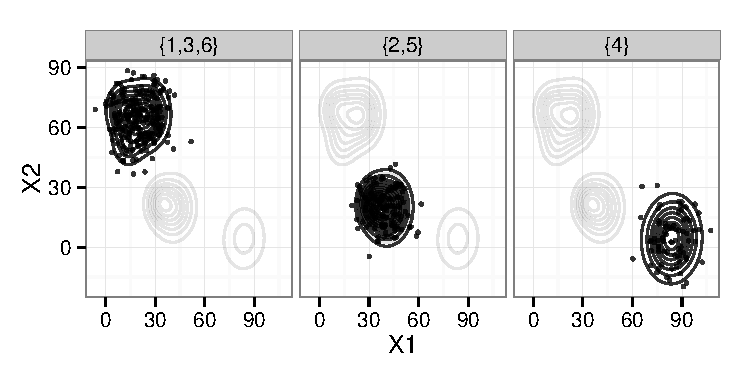
\includegraphics[trim=0cm 0cm 0cm 0cm,width=0.5\textwidth]{figures/partition-example-part3a.pdf} \\
          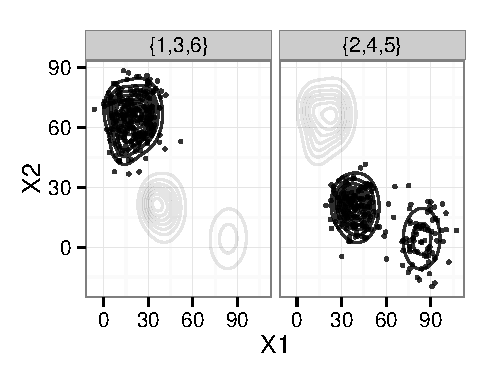
\includegraphics[trim=0cm 0cm 0cm 0cm,width=0.33\textwidth]{figures/partition-example-part2.pdf} \\
            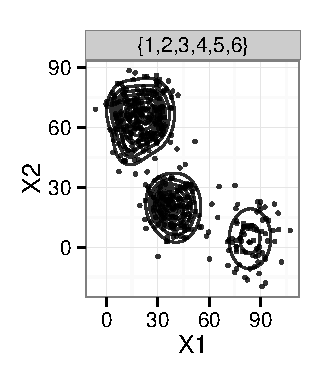
\includegraphics[trim=0cm 0cm 0cm 0cm,width=0.2\textwidth]{figures/partition-example-part1.pdf}
 \end{tabular}
 \caption{Hierarchical cluster obtained by the hierarchical combination of components.}\label{hierarchical}
\end{center}
\end{figure}

In this article, we are not interested in how to decide which of the different partitions in a hierarchical combination of components defines a ``better'' clustering. Instead, we propose different methods to decide how to merge the components. More concretely, given a finite mixture we are interested in analysing methods to decide how to merge components only using information given by the posterior probabilities $\hat{\tau}_{i \mathcal{I}}$, $1\leq i \leq n$.


\section{Hierarchical algorithms based on posterior probabilities}

Using definitions given in Section~\ref{definitions} we revisite some Hierarchical algorithms based on posterior probabilities from the literature

\subsection*{Algorithm based on the total Entropy}

%Let ${\boldsymbol\tau}_1, \dots, {\boldsymbol\tau}_n$ be the probability vectors giving the probability that elements $\textbf{x}_1, \dots, \textbf{x}_n$ belongs to classes $C_1, \dots, C_k$.  

\cite{baudry2010combining} proposes the  hierarchical combination of components  $\mathcal{I}_1, \dots, \mathcal{I}_k$ defined as follows: starting from partition $\mathcal{I}_k = \{\{1\},\dots, \{k\}\}$ at each step the method combines two parts. If at current step we have the partition  $I_1, \dots, I_s$ the two parts, $I_a, I_b$, $1 \leq a,b \leq s$, to be combined are those that maximise the entropy criterion

\[
- \sum_{i=1}^n \left\{ \hat{\tau}_{iI_a} \log(\hat{\tau}_{iI_a}) + \hat{\tau}_{iI_b} \log(\hat{\tau}_{iI_b})\right\} +  \sum_{i=1}^n  (\hat{\tau}_{iI_a}+\hat{\tau}_{iI_b}) \log(\hat{\tau}_{iI_a} + \hat{\tau}_{iI_b}),
\]

or equivalently,

\[
 \sum_{i=1}^n \hat{\tau}_{i I_a \cup I_b} \log(\hat{\tau}_{i I_a \cup I_b}) - \hat{\tau}_{iI_a} \log(\hat{\tau}_{iI_a}) - \hat{\tau}_{iI_b} \log(\hat{\tau}_{iI_b}).
\]

{\color{red} Dir que la idea equival a la variació en entropies de Shannon en fer la fusió  i que l'entropia no és més que una dissimilitud entre la full composition i el centre del simplex.}
%in other words $\dots$

\subsection*{DEMP algorithm}

%Let ${\boldsymbol\tau}_1, \dots, {\boldsymbol\tau}_n$ be the probability vectors giving the probability that elements $\textbf{x}_1, \dots, \textbf{x}_n$ belongs to classes $C_1, \dots, C_k$. 

DEMP approach \citep{hennig2010methods} proposes the hierarchical combination of components  $\mathcal{I}_1, \dots, \mathcal{I}_k$ defined as follows: starting from partition $\mathcal{I}_k = \{\{1\},\dots, \{k\}\}$ at each step the method combines two parts. If at current step we have the partition  $I_1, \dots, I_s$ the two parts, $I_a, I_b$, $1 \leq a,b \leq s$,  to be combined are those that maximise the misclassification probabilities estimated by 

\begin{equation}\label{demp_criteria}
\frac{ \frac{1}{n} \sum_{i=1}^n {\hat{\tau}_{iI_a} \mathbbm{1}_{\left[ \forall j\; \hat{\tau}_{i I_{b}} \geq \hat{\tau}_{iI_j} \right]}}}{ \hat{\pi}_{I_a}}.
\end{equation}

The function indicator $\mathbbm{1}_{\left[ \forall j\; \hat{\tau}_{i I_{b}} \geq \hat{\tau}_{iI_j} \right]}$ is defined by
\[
\mathbbm{1}_{\left[ \forall j\; \hat{\tau}_{i I_{b}} \geq \hat{\tau}_{iI_j} \right]} =
\left\{\begin{array}{ll}	
1 & \text{if $\forall j\; \hat{\tau}_{i I_{b}} \geq \hat{\tau}_{iI_j}$}\\
0 & \text{if $\exists j\; \hat{\tau}_{i I_{b}} < \hat{\tau}_{iI_j}$}
\end{array}\right.
\]
{\color{red} Martin diu que potser hauria de ser $a$ a sota.  Diria que no.}
{\color{red} Dir què és el DEMP i com mesura la confusió entre b i a. En Hennig parla de misclassification}

\subsection*{The log-ratio algorithm}

The log-ratio approach \citep{ComasCufi2013} proposes the hierarchical combination of components $\mathcal{I}_1, \dots, \mathcal{I}_k$ defined as follows: starting from partition $\mathcal{I}_k = \{\{1\},\dots, \{k\}\}$ at each step the method combines two parts. If at current step we have the partition  $I_1, \dots, I_s$ the two parts, $I_a, I_b$, $1 \leq a,b \leq s$,  to be combined are those that \emph{minimise} log-ratio criterion by

\[
\frac{\sum_{i=1}^n \mathbbm{1}_{\left[ \forall j\; \hat{\tau}_{i I_{a}} \geq \hat{\tau}_{iI_j} \right]} \log( \frac{ \hat{\tau}_{iI_a} }{ \hat{\tau}_{iI_b} })}{\sum_{i=1}^n \mathbbm{1}_{\left[ \forall j\; \hat{\tau}_{i I_{a}} \geq \hat{\tau}_{iI_j} \right]}}.
\]

When the log-ratio algorithm was proposed, the authors wanted to incorporate two idea

{\color{red} Dir que la mesura és igual a la mitjana de les distàncies entre la subcomposició $(\tau_a, \tau_b)$ i $(0.5,0.5)$ per les observacions classificades a $a$.}

\begin{itemize}
\item a local measure of how possible is to confuse $I_b$ with $I_a$ depending on each observation $\m x_i$, $\log( \frac{ \hat{\tau}_{iI_a} }{ \hat{\tau}_{iI_b} })$, and
\item a measure of how associated is an observation $\m x_i$ to cluster $I_a$, $\mathbbm{1}_{\left[ \forall j\; \hat{\tau}_{i I_{a}} \geq \hat{\tau}_{iI_j} \right]}$.
\end{itemize}

\section{Unifying the approaches}

In this section, we extend the ideas that motivate the log-ratio algorithm to a general framework. We consider a local measure given by function $\lambda(\hat{\m\tau}_{i \mathcal{I}}, I, J)$ of how similar are the clusters given by part $I$ and part $J$ in $\m x_i$, and a measure of how associated is an observation $\m x_i$ to the cluster given by part $I$, $\omega(\m x_i, I)$. This general approach proposes the hierarchical combination of components $\mathcal{I}_1 \dots, \mathcal{I}_k$ defined as follows: starting from partition $\mathcal{I}_k = \{\{1\},\dots, \{k\}\}$ at each step the method combine two parts. If at current step we have the partition  $I_1, \dots, I_s$ the two parts, $I_a, I_b$, $1 \leq a,b \leq s$,  to be combined are those that \emph{minimise} the general criterion given by

\begin{equation}
\frac{\sum_{i=1}^n \omega(\hat{\tau}_{i \mathcal{I}_s}, I_a) \lambda(\hat{\tau}_{i \mathcal{I}_s}, I_a, I_b)}{\sum_{i=1}^n \omega(\hat{\tau}_{i \mathcal{I}_s}, I_a) }.
\end{equation}

For example, in the log-ratio algorithm $\lambda(\hat{\tau}_{i \mathcal{I}_s}, I_a, I_b)$ and $\omega(\m x_i, I_a)$ are defined as follows
\[
\lambda(\hat{\tau}_{i \mathcal{I}_s}, I_a, I_b) = \log( \frac{ \hat{\tau}_{iI_a} }{ \hat{\tau}_{iI_b} })
\]
and
\[
\omega(\hat{\tau}_{i \mathcal{I}_s}, I_a) = \mathbbm{1}_{\left[ \forall j\; \hat{\tau}_{i I_{a}} \geq \hat{\tau}_{iI_j} \right]}.
\]
In the log-ratio algorithm $\log( \frac{ \hat{\tau}_{iI_a} }{ \hat{\tau}_{iI_b} })$ plays the role of measuring how different are partition $I_a$ and $I_b$ using the posterior probabilities $\hat{\tau}_{i \mathcal{I}_s}$ of observation $\m x_i$. By contrast, $\mathbbm{1}_{\left[ \forall j\; \hat{\tau}_{i I_{a}} \geq \hat{\tau}_{iI_j} \right]}$ plays the role of how important is observation $\m x_i$ in the decision of asserting the differences of partition $I_a$ and $I_b$.

The following three propositions state that the algorithm based on the total Entropy, the DEMP algorithm and the log-ratio algorithm can be formulated with the general criterion with suitable definitions for $\lambda(\hat{\tau}_{i \mathcal{I}_s}, I_a, I_b)$ and $\omega(\hat{\tau}_{i \mathcal{I}_s}, I_a)$.

{\color{red} Canviar les proposicions a explicacions a dins del text}
\begin{prop}
The hierarchical combination of components given by the general approach with
\[
\lambda(\hat{\tau}_{i \mathcal{I}_s}, I_a, I_b) = \hat{\tau}_{iI_b} \log(\hat{\tau}_{iI_b}) + \hat{\tau}_{iI_a} \log(\hat{\tau}_{iI_a}) - \hat{\tau}_{i I_a \cup I_b} \log(\hat{\tau}_{i I_a \cup I_b})
\]
and
\[
\omega(\hat{\tau}_{i \mathcal{I}_s}, I_a) = const
\]
is the same as the one obtained with the total Entropy algorithm.
\end{prop}
\begin{proof}
Maximising
\[
\sum_{i=1}^n \hat{\tau}_{i I_a \cup I_b} \log(\hat{\tau}_{i I_a \cup I_b}) - \hat{\tau}_{iI_a} \log(\hat{\tau}_{iI_a}) - \hat{\tau}_{iI_b} \log(\hat{\tau}_{iI_b}).
\]
respect to $I_a$ and $I_b$ is equivalent to minimise
\begin{equation}\label{min_entropy}
\sum_{i=1}^n \hat{\tau}_{iI_a} \log(\hat{\tau}_{iI_a}) + \hat{\tau}_{iI_b} \log(\hat{\tau}_{iI_b}) - \hat{\tau}_{i I_a \cup I_b} \log(\hat{\tau}_{i I_a \cup I_b}).
\end{equation}
respect to $I_a$ and $I_b$. Multiplying by a constant does not change the result of an optimisation problem. Therefore, multiplying by $\frac{1}{n}$ Eq.~\ref{min_entropy} can be written as
\[
\frac{\sum_{i=1}^n const \; ( \hat{\tau}_{iI_a} \log(\hat{\tau}_{iI_a}) + \hat{\tau}_{iI_b} \log(\hat{\tau}_{iI_b}) - \hat{\tau}_{i I_a \cup I_b} \log(\hat{\tau}_{i I_a \cup I_b}) )}{\sum_{i=1}^n const}.
\]
\end{proof}

\begin{prop}
The hierarchical combination of components given by the general approach with
\[
\lambda(\hat{\tau}_{i \mathcal{I}_s}, I_a, I_b) = \mathbbm{1}_{\left[ \exists j\; \hat{\tau}_{i I_{b}} < \hat{\tau}_{iI_j} \right]}
\]
and
\[
\omega(\hat{\tau}_{i \mathcal{I}_s}, I_a) = \hat{\tau}_{iI_a}
\]
is the same as the one obtained with the DEMP algorithm.
\end{prop}
\begin{proof}
Because $\hat{\pi}_{I_a}$ is estimated as $\hat{\pi}_{I_a} = \sum_{i=1}^n \hat{\tau}_{iI_a}$, Eq.~\ref{demp_criteria} is equivalent to
\begin{equation}\label{demp_criteria_taus}
\frac{ \sum_{i=1}^n {\hat{\tau}_{iI_a} \mathbbm{1}_{\left[ \forall j\; \hat{\tau}_{i I_{b}} \geq \hat{\tau}_{iI_j} \right]}}}{  \sum_{i=1}^n \hat{\tau}_{iI_a}}.
\end{equation}
Maximising Eq.~\ref{demp_criteria_taus} with respect to $I_a$ and $I_b$ is equivalent to minimise
\[
\frac{ \sum_{i=1}^n {\hat{\tau}_{iI_a} \mathbbm{1}_{\left[ \exists j\; \hat{\tau}_{i I_{b}} < \hat{\tau}_{iI_j} \right]}}}{  \sum_{i=1}^n \hat{\tau}_{iI_a}}.
\]
respect to $I_a$ and $I_b$.
\end{proof}

\begin{prop}
The hierarchical combination of components given by the general approach with
\[
\lambda(\hat{\tau}_{i \mathcal{I}_s}, I_a, I_b) = \log( \frac{ \hat{\tau}_{iI_a} }{ \hat{\tau}_{iI_b} })
\]
and
\[
\omega(\hat{\tau}_{i \mathcal{I}_s}, I_a) =<\mathbbm{1}_{\left[ \forall j\; \hat{\tau}_{i I_{a}} \geq \hat{\tau}_{iI_j} \right]}
\]
is the same as the one obtained with log-ratio algorithm.\qed
\end{prop}

{\color{red} Aquest paràgraf està molt "xulo". Però crec que cal haver-ne parlat abans quan s'ha presentat els índexos. 
Vull dir, quan es presetna cada índex aniria bé explicar la idea "geomètrica" que ha pensat l'autor (Henning,  Baudry, Comas). Després aquí, aquest aparta xulo s'entendrà molt més. }


The three algorithms give us three different possible definition for functions $\lambda(\hat{\tau}_{i \mathcal{I}_s}, I_a, I_b)$ and $\omega(\hat{\tau}_{i \mathcal{I}_s}, I_a)$. For the function $\lambda(\hat{\tau}_{i \mathcal{I}_s}, I_a, I_b)$ the entropy algorithm considers that the more the confusion is between two parts the higher is the difference between the entropy considering the partition with the two part together and merged. The way the confusion is defined by the DEMP algorithm is more subtle, it states that the higher the confusion between two parts the higher the number of observations not classified to one part. The log-ratio approach relates the confusion respect to the magnitude of the log-ratio. For the function $\omega(\hat{\tau}_{i \mathcal{I}_s}, I_a)$, the entropy algorithm weighs equally the local information of each observation to decide if $I_a$ should be merged to $I_b$. By contrast, the DEMP algorithm weighs the observation according to the probability of pertinence to $I_a$. Finally, the log-ratio algorithm weighs with respect the final pertinence to $I_a$.

{\color{red} Seguir l'exemple de les 6 components i estudiar com es calculen els tres indexos en un determinat pas de la jerarquia. Per exemple, quan es decideix fusion el {3} amb el {1,6}. O alguna cosa simila. Preparar-ho pel CoDaWor juntament amb un cas d'estudi final}

{\color{red} Posar lo de Kullback Leibler prenent tau i logratio. Donar la idea que no només és una unificació de tres index si no que una generalització.}

\bibliographystyle{apalike}
\bibliography{tex/combining_mixtures}{}

\end{document}
